\documentclass[12pt,a4paper]{amsart}
%\usepackage[norsk]{babel}
\usepackage[english]{babel}
\usepackage[utf8]{inputenc}
%\usepackage[fleqn]{amsmath}
\usepackage{amsmath}
\usepackage[T1]{fontenc}
\usepackage{mathtools}
\usepackage{graphicx}
\usepackage{subcaption}
\usepackage{verbatim}
\usepackage{listings}
\usepackage{scalerel}
\usepackage{fixltx2e}
\usepackage{amssymb}
\usepackage{siunitx}
\usepackage{xfrac}
\usepackage{enumitem}
\usepackage{hyperref}
\usepackage{float}
\usepackage{bbold}
\usepackage{physics}
\usepackage[ampersand]{easylist}
\usepackage{subcaption}
\usepackage{wrapfig}
\usepackage{algorithmicx}
\usepackage{csquotes}
\usepackage{xcolor}

%%For visualizations of table
\usepackage{multirow}
\usepackage{arydshln}
\usepackage{booktabs}

%% References section
\usepackage[english]{babel}\addto\captionsenglish  
{\renewcommand{\bibname}{References}}  
\usepackage[backend=bibtex,style=phys]{biblatex}  %backend=biber is 'better'  
%\usepackage[backend=biber]{biblatex}
%\usepackage{apacite}
\addbibresource{Higgs_analysis.bib}

\usepackage[margin=1.5in]{geometry}
\newcommand{\scalel}{\scaleleft{<}}
\newcommand{\scaler}{\scaleright{>}}

%% physics packages
\usepackage{physics}
\usepackage[compat=1.1.0]{tikz-feynman}
\usepackage{feynmf}

% adjust the spacing around figure if pdf-file with white space:
\usepackage[font=small,skip=0pt]{caption}
%\usepackage[margin=1.4in]{geometry}
%\captionsetup[figure]{skip=-100pt}

% define colors for text
\definecolor{mygreen}{RGB}{28,172,0} % color values Red, Green, Blue
\definecolor{mylilas}{RGB}{170,55,241}
\definecolor{forestgreen}{rgb}{0.13, 0.55, 0.13}

% definitions of commands
%\renewcommand{\thesection}{\arabic{section}}

%\makeatletter
%\patchcmd{\@settitle}{\uppercasenonmath\@title}{}{}{}
% layout for sections, subsections and subsubsections
%\usepackage{titlesec} % Allows customization of titles
%\renewcommand\thesection{\Roman{section}} % Roman numerals for the sections
%\renewcommand{\thesubsection}{\Alph{subsection}} % Alphabetic letters for the subsections
%\renewcommand{\thesubsubsection}{\arabic{subsubsection}} % Arabic numerals for the subsubsections
%\titleformat{\section}[block]{\normalfont\scshape\centering\bfseries}{\thesection.}{1em}{} % Change the look of the section titles
%\titleformat{\subsection}{\normalsize\large\filcenter\bfseries}{\thesubsection.}{1em}{}
%\titleformat{\subsubsection}[runin]{\medium\bfseries}{\thesubsubsection.}{1em}{}% Change the look of the section titles

\title[Higgs analysis walkthrough]{Higgs Analysis Walkthrough\\
\small{\mdseries Data Analysis in High Energy Physics}}
\date{\today}
\author[Christensen]{Elisabeth Christensen}

\begin{document}
\maketitle

\begin{abstract}
Provided invariant mass distributions of the background and signal samples for the process $H\rightarrow 4\mu$, along with a mass distribution for observed data, we investigate the luminosity scale factor required for the discovery of a signal on top of the SM background, and the discovery and exclusion limits of the current dataset without an increase of the luminosity. We also look at the optimal mass window and the scalefactors needed to account for any systematic effects caused by the nuisance parameters for the background and signal samples using MLE.
\end{abstract}

\section{Introduction}\label{sec:introduction}
In order to claim discovery of a hypothetical particle, the groundwork of the search for the particle must first be made. The main, and most widely used, approach in doing so is through the application of statistical physics, which gives us the tool of predicting the possible existence of a particle. We will throughout this project take a look at the discovery of the Higgs boson decaying to a 4-muon final state. The statistical methods, discussed further below, used in the search for the Higgs boson at an invariant mass of 125GeV will be applied to pseudo-datasets (fake data). The background, $H_0$, is based on the Standard Model of particle physics and includes the decay of two Z-bosons to the 4-muon final state. In the first part we will try to optimize the expected significance by improving the range of the mass-window used for the counting of events in the invariant mass distribution (figure~\ref{fig:mass_distribution_mll}). We will also investigate the lower boundary of the luminosity scale factor needed for an expected significance of approximately $5\sigma$. Second, we will look into the effects of systematic uncertainties in the MC datasets for the background and signal samples by investigating the nuisance parameters in both background and signal. From this we can try to estimate the scalefactors needed using a maximum-likelihood estimate (MLE) through a side-band fit. Finally, we will create MC toy-datasets in order to find the median test-statistic of the $H_0$ (background only, or b-only) and $H_1$ (signal+background, or $s+b$) hypotheses, using the likelihood-ratio as the test-statistic. We will also compute the confidence levels under both the b-only and $s+b$ hypotheses.

\begin{figure}
\centering
\includegraphics[width=.8\textwidth]{../data/11_1/MassPlot_rebin20.pdf}
\caption{4-lepton invariant mass distribution of signal $H\rightarrow 4\mu$, background $ZZ\rightarrow 4\mu$ and observed data.}
\label{fig:mass_distribution_mll}
\end{figure}

\section{Theory and Methods} \label{sec:theory_and_methods}
\subsection{Frequentist approach} \label{subsec:theory_frequentist_approach}
Prompting the search for the Higgs boson we will make use of what is known as the frequentist approach. This approach relies on repeating an experiment multiple times with the same initial conditions. In doing so we can calculate what is known as the p-value, which allows us to determine the probability of obtaining results as extreme as the observed results \textit{given} that $H_0$ is true. The p-value let us in turn calculate the significance of our expected results.

\subsubsection{P-values and significance} \label{subsec:Theory-p-values_and_significance}
The p-value is defined by the cut made for the signal region and thus depends on the test-statistic $t_C$ for this critical region~\cite{Behnke_2015:Data_analysis_in_HEP}. The p-value can be expressed in terms of the probability density function (pdf) $g(t|H_i)$ where $H_i$ can correspond to either the background hypothesis $H_0$ or the signal+background hypothesis $H_1$.

\begin{align}
p_i = \int_{t_{obs}}^{+\infty} g(t|H_i)dt	\label{eq:p_value_continuos}
\end{align}
Here, $t_{obs}$ corresponds to the observed test-statistic\footnote{This is often taken as either the number of events counted or the log-likelihood ratio.}.
A counting experiment, such as ours, can be well represented by the Poisson distribution, which is the limit of the binomial distribution. Thus, the p-values used in our analysis under $H_0$ and $H_1$ is defined as

\begin{align}
\begin{split}
	p_0 &= \sum_{n=n_{obs}}^\infty f(n;b) = \sum_{n=n_{obs}}^\infty \frac{b^n}{n!}e^{-b} \label{eq:p_value_discrete_poisson}\\
	p_1 &= \sum_{n=n_{obs}}^\infty f(n;s+b) = \sum_{n=n_{obs}}^\infty \frac{(s+b)^n}{n!}e^{-(s+b)}
\end{split}
\end{align}
with $n_{obs}$ equal to the total number of observed events.

According to the central limit theorem, the Poisson distribution can be approximated as a normal distribution for a large number of events. In such a case the significance can be related to the p-value using a unit Gaussian, i.e.

\begin{align}
p = \int_Z^\infty\frac{1}{2\pi} e^{\frac{1}{2}t^2}dt \hspace{.25cm} \Longrightarrow \hspace{.25cm} Z = \Phi^{-1}(1-p)\label{eq:significance}
\end{align}
where $\Phi^{-1}$ is the cumulative distribution function of the unit Gaussian. 

\subsubsection{Likelihood} \label{susubsec:Theory-p-values_and_significance-likelihood}
The likelihood is defined as
\begin{align}
\mathcal{L}(\mu_s, \alpha_{bgr}) = \prod_{\text{bins i}}f(n_i; \alpha_{bgr}b_i + \mu_{s}s_i) \label{eq:likelihood}
\end{align}
where $\alpha_{bgr}$ and $\mu_s$ corresponds to the scalefactors needed to account for nuisance parameters for the background and signal events, respectively. $f$ corresponds to the invariant mass distribution for a 4-lepton final state and is defined as
\begin{align}
f(m_{4l}) = \alpha_{bgr} \cdot f_{SM}(m_{4l}) + \mu_s\cdot f_{Higgs}(m_{4l}) \label{eq:invariant_mass_dist_m_4l}
\end{align}
with $f_{SM}$ and $f_{Higgs}$ corresponding to the expected distribution of events in the background and signal samples. In order to find the optimum scalefcators one can utilize the maximum likelihood estimate from the log-likelihood, i.e.
\begin{align}
\ln \mathcal{L}(\alpha_{bgr}, \mu_s) &= \sum_{\text{bins i}}\ln f(n_i; \alpha_{bgr}b_i + \mu_{s}s_i) \label{eq:logL}
\end{align}
For a given nuisance parameter $\theta$ the MLE is estimated as
\begin{align}
\frac{\partial \ln \mathcal{L}}{\partial \theta} = 0 \label{eq:MLE}
\end{align}

The uncertainty on the scalefactors can be found using the contour given by a range of values $\mathbf{ \theta}'$ with the demand that the difference of the scaled log-likelihood and its maximum value is equal to $-\frac{1}{2}$.

\begin{align}
\Delta \ln \mathcal{L} \equiv \ln \mathcal{L}(\bold{\theta}') - \ln \mathcal{L}_{max} = -\frac{1}{2}
\end{align}

\subsubsection{Test-statistic} \label{subsubsec:Theory-(p-values and significance)-(test-statistic)}
The test-statistic allows us to determine the level of agreement of a hypothesis with the observation and is often defined as either the number of events counted or the log-likelihood ratio of the $H_1$ hypothesis vs. the $H_0$ hypothesis. In other words, the test statistic evaluates how much less (or more) likely data under the null-hypothesis are able to account for the observed data compared to the data provided by the $s+b$ hypothesis. The test-statistic can in simple terms be expressed as
\begin{align}
t = -2\ln\frac{\mathcal{L}(\mu=1)}{\mathcal{L}(\mu=0)} = 2[\ln\mathcal{L}(x|H_0) - \ln\mathcal{L}(x|H_1)] \label{eq:test_statistic},
\end{align}
where the likelihood $\mathcal{L}$ is the same as that of eq.~\eqref{eq:likelihood}.

\subsubsection{Confidence levels} \label{subsubsec:Theory-(p-values and significance)-(confidence-levels)}
Towards the end of an analysis, one major question yet remains, and requires a reliable answer based on the evidence provided. This is the question of whether or not one can claim a discovery based on the significance of the signal sample or if one must exclude the $s+b$ hypothesis due to the incompatibility with the observed data. Confidence levels provides an extra step along the way in confirming or excluding our theoretical model for $H_1$.
They allow us to determine the probability of measuring the observed test-statistic, $t_{obs}$, given that either $H_0$ or $H_1$ is true. We have two different definitions of the confidence level regarding which scheme we're looking at. If we are interested in the probability of whether or not the test-statistic under the b-only hypothesis is as small or smaller than $t_{obs}$, which would imply a more signal-like distribution, then we could use the confidence level $1-CL_b$. If we however are more interested in the probability for the test-statistic to be as large or larger than $t_{obs}$ under the $s+b$ hypothesis then we could use the confidence level known as $CL_{s+b}$ to describe such a probability. The confidence levels in the two different regimes are defined as
\begin{align}
1-CL_b &= \int_{-\infty}^{t_{obs}} g(t;\text{b-only)})dt \label{eq:1-CL_b}\\
CL_{s+b} &= \int_{t_{obs}}^\infty g(t;s+b)dt	\label{eq:CL_s+b}
\end{align}
However, using these estimates does not necessarily tell us whether or not we can exclude the signal-only hypothesis. This is mainly due to the potential overlapping of pdf's. If e.g. the signal is small or the analysis is not powerful enough to separate signal and background, then the pdf's can overlap. In such a case saying that $CL_s \approx CL_{s+b}$ can lead to confusion and misinterpretation of the result itself, as it gives us an incorrect estimate on the true exclusion level of the signal when the background is contaminating the region. Since we are interested in whether or not we can exclude the signal-only hypothesis we can use the $CL_s$ method\cite{Read_2002:CLs}, which in itself is not strictly a true frequentist confidence level, but displays more Bayesian-like properties as it allows us to determine the upper limit of counting experiments in the presence of background events. Rather than stating the probability that $m_H > m_{\hat{H}}$ is $95\%$ for a mass limit $m_{\hat{H}}$, which is exclusively reserved the Bayesian intepretation in terms of the posterior probability, we can instead say that if $CL_s(m_H) \leq 5\%$ for a given mass $m_H$, then we can exclude any $m_H \leq m_{\hat{H}}$ with a $95\%$ certainty. 
Using the b-only and $s+b$ confidence levels we can construct what is known as $CL_s$, i.e. the ratio of the two confidence levels:
\begin{align}
CL_s = \frac{CL_{s+b}}{CL_b}	\label{eq:CL_s}
\end{align}
\begin{itemize}
\item \textit{Discovery}: Discovery implies that the significance indicated by the p-value must be equal to or less than $5\sigma$. 
\item \textit{Exclusion}: Using the confidence level ratio $CL_s$ we can determine whether or not the $H_1$ hypothesis should be excluded. That is, if $CL_s < 5\%$ then we can exclude $H_1$ with a $95\%$ confidence level.
\end{itemize}

\section{Analysis} \label{sec:Analysis}
\subsection{Optimizing the mass window} \label{subsec:Analysis-(optimizing_the_mass_window)}
The mass window is optimised by testing a range of symmetric widths around the theoretical invariant mass of 125 GeV. The mass windows range from 0-25 GeV. Using eq.~\eqref{eq:significance} we can find the expected (and observed) significance for each mass window. The distribution of the significance vs. the mass window is seen in figure~\ref{fig:mass_windows_significance_lumFactor=1}. Here, the maximum for the expected significance is $2.04\sigma$ which implies a mass window of $125\pm 7.15$ GeV, while the maximum for the observed significance is $3.92\sigma$ as a result of using a mass window of $125 \pm 2.85$ GeV. The observed significance should however not be used any further throughout this analysis as it might cause a significant bias in our data by no longer treating it as a \textit{blind analysis}. The values mentioned are summarised in table~\ref{tab:Significance_vs_lumScaleFactors}.

The effect of an increased luminosity using a scalefactor of 5 can be seen in figure~\ref{fig:mass_windows_significance_lumFactor=5}. The maximum of the expected significance for an enhanced luminosity now results in $Z = 4.79$ using a mass window of $125\pm6.55$ GeV. The observed significance was only used as a demonstration in the previous example and as it will not be included in any further work, it is ignored in this figure.

\begin{figure*}[t!]
    \centering
    \begin{subfigure}[t]{0.6\textwidth}
        \centering
        \includegraphics[width=1\textwidth]{../data/11_1/Significance_Optimization_lumiscalefactor_1_00.pdf}
        \caption{Luminosity scalefactor = 1.00.}
		\label{fig:mass_windows_significance_lumFactor=1}
    \end{subfigure}%
    ~ 
    \begin{subfigure}[t]{0.6\textwidth}
        \centering
        \includegraphics[width=1\textwidth]{../data/11_1/Significance_Optimization_lumiscalefactor_5_00.pdf}
        \caption{Luminosity scalefactor = 5.00.}
    		\label{fig:mass_windows_significance_lumFactor=5}
	\end{subfigure}
	\caption{Observed and expected significance vs. mass window, using (A) a luminosity scalefactor of 1 and (B) a luminosity scalefactor of 5.}
\label{fig:mass_windows_significance}
\end{figure*}

The effect of an enhanced luminosity is reflected in figure~\ref{fig:significance_vs_lumScaleFactors}. Here, the optimum significance is found for a certain luminosity scalefactor as before using a range of possible mass windows. In order to claim a discovery one needs a p-value < $5.73\times 10^{-7}$, or, in other words, a significance equal to or greater than $5\sigma$. The lower threshold for the luminosity required in order to claim discovery is a scalefactor of 5.40, resulting in a significance of $5.02\sigma$.

\begin{figure}
\centering
\includegraphics[width=0.8\textwidth]{../data/11_1/Luminosity_scalefactors_vs_optimum_significance.pdf}
\caption{Optimum expected significance vs. luminosity scale factors. The lower bound of luminosity scale factor needed is marked by the horizontal, dashed line.}
\label{fig:significance_vs_lumScaleFactors}
\end{figure}

\begin{table}[]
\caption{Optimum significances, by the comparing of mass windows, for variable luminosity scalefactors (sf) ranging from 0 to 7.}
\label{tab:Significance_vs_lumScaleFactors}
\begin{tabular}{c|cc}
\hline\hline
Lum. sf & Mass win. [GeV] & $Z_{exp} [\sigma]$ \\ \hline
1.00             &7.15      & $2.04$  \\
5.00             & 6.55      & $4.79$ \\
5.40             & 6.35      & $5.02$ \\ \hline\hline
\end{tabular}
\end{table}

\subsection{Background estimate: sideband fits} \label{subsec:Analysis-(background estimate:sideband fits)}
In order to perform as close to an unbiased analysis as one can come, we choose to look outside the signal region and optimise the bacgkround and signal nuisance parameters based on the sideband region, in an attempt to avoid possible systematic effetcs. The region we will be focusing on is defined to be $150\leq m_H \leq 400$ GeV. Using the MLE from eq.~\eqref{eq:MLE} we can find the optimal scalefactor $\alpha_{bgr}$ for the background sample. Using the optimal mass window found previously we find that the number of background events is $b = 4.64$. The optimal scalefactor $\alpha_{bgr}$ thus becomes 
\begin{align*}
\alpha_{bgr} = 1.11^{+0.07}_{-0.06}
\end{align*}
and is illustrated along with the log-likelihood in figure~\ref{fig:background_scalefactor}.
\begin{figure}
\centering
\includegraphics[width=0.8\textwidth]{../data/11_2/SideBand_fit.pdf}
\caption{$\alpha_{bgr}$ vs- $-2\log(\mathcal{L})$ where the red line represents to the optimal $\alpha_{bgr}$ with purple lines representing the corresponding $\alpha_{bgr}$ errors.}
\label{fig:background_scalefactor}
\end{figure}
While using a mass window of $7.15$ GeV and a luminosity scalefactor of 1, the scaled number of background events $b_{scale}$ with corresponding uncertainties becomes
\begin{align*}
b = 4.64 \hspace{.2cm }\Longrightarrow \hspace{.2cm} b_{scale} = 5.13^{+0.31}_{-0.29}
\end{align*}

Using $b_{scale}$ as our new background estimate we can calculate the expected and observed significance by generating MC toy datasets. This is done by drawing a random number of events according to the Poisson distribution with the mean taken as the number of background events ($b_{scale}$-only) and the number of signal+background events ($s+b_{scale})$. When drawing the random number of events around $b_{scale}$ we do so using a random number generator on the gaussian distribution, as the Poisson distribution can be approximated to a normal distribution when dealing with large quantities, whereas the random number of signal events is drawn from the Poisson distribution. In doing so, our new expected and observed significance now becomes
\begin{align*}
&(\Delta b_{scale} = 0): \hspace{.5cm} Z_{exp} = 1.90,\hspace{.5cm} Z_{obs} = 2.80 \\
&(\Delta b_{scale} \neq 0): \hspace{.5cm} Z_{exp} = 1.90,\hspace{.5cm} Z_{obs} = 2.80 \\
\end{align*}
We can see that when incorporating the uncertainty on the new scaled background the significances stay the same, i.e. the impact of the uncertainty on $b_{scale}$ is negligible. As the number of background events increase by approximately $11\%$ the expected and observed significances becomes lower due to the fact that the background is now able to account for the smaller previous discrepancies between the number events observed vs. the number events explained by the background. The same goes for the observed significance which has decreased from the previous value of $3.92\sigma$ under the b-only hypothesis.

Taking it one step further we can calculate the optimal scale factors $\mu_s$ and $\alpha_{bgr}$ from eq.~\eqref{eq:invariant_mass_dist_m_4l} simultaneously. We do this by computing a grid on two ranges of $\alpha_{bgr}$ and $\mu_s$, as before, and compute $-2\log(\mathcal{L})$ before storing the values in a 2D-histogram with a rebin factor of 10, i.e. 10 times wider bins. The minimum of $-2\log(\mathcal{L})$ thus corresponds to the optimal scale factors. From figure~\ref{fig:optimal_scalefactors_contourPlot} the minimum value of $-2\log(\mathcal{L})$ is marked with a white star, which corresponds to the scale factors.

\begin{align*}
\alpha_{bgr} = 1.11^{+0.07}_{-0.06}, \hspace{.5cm} \mu_s = 1.29^{+0.64}_{-0.54}
\end{align*}

\begin{figure}
\centering
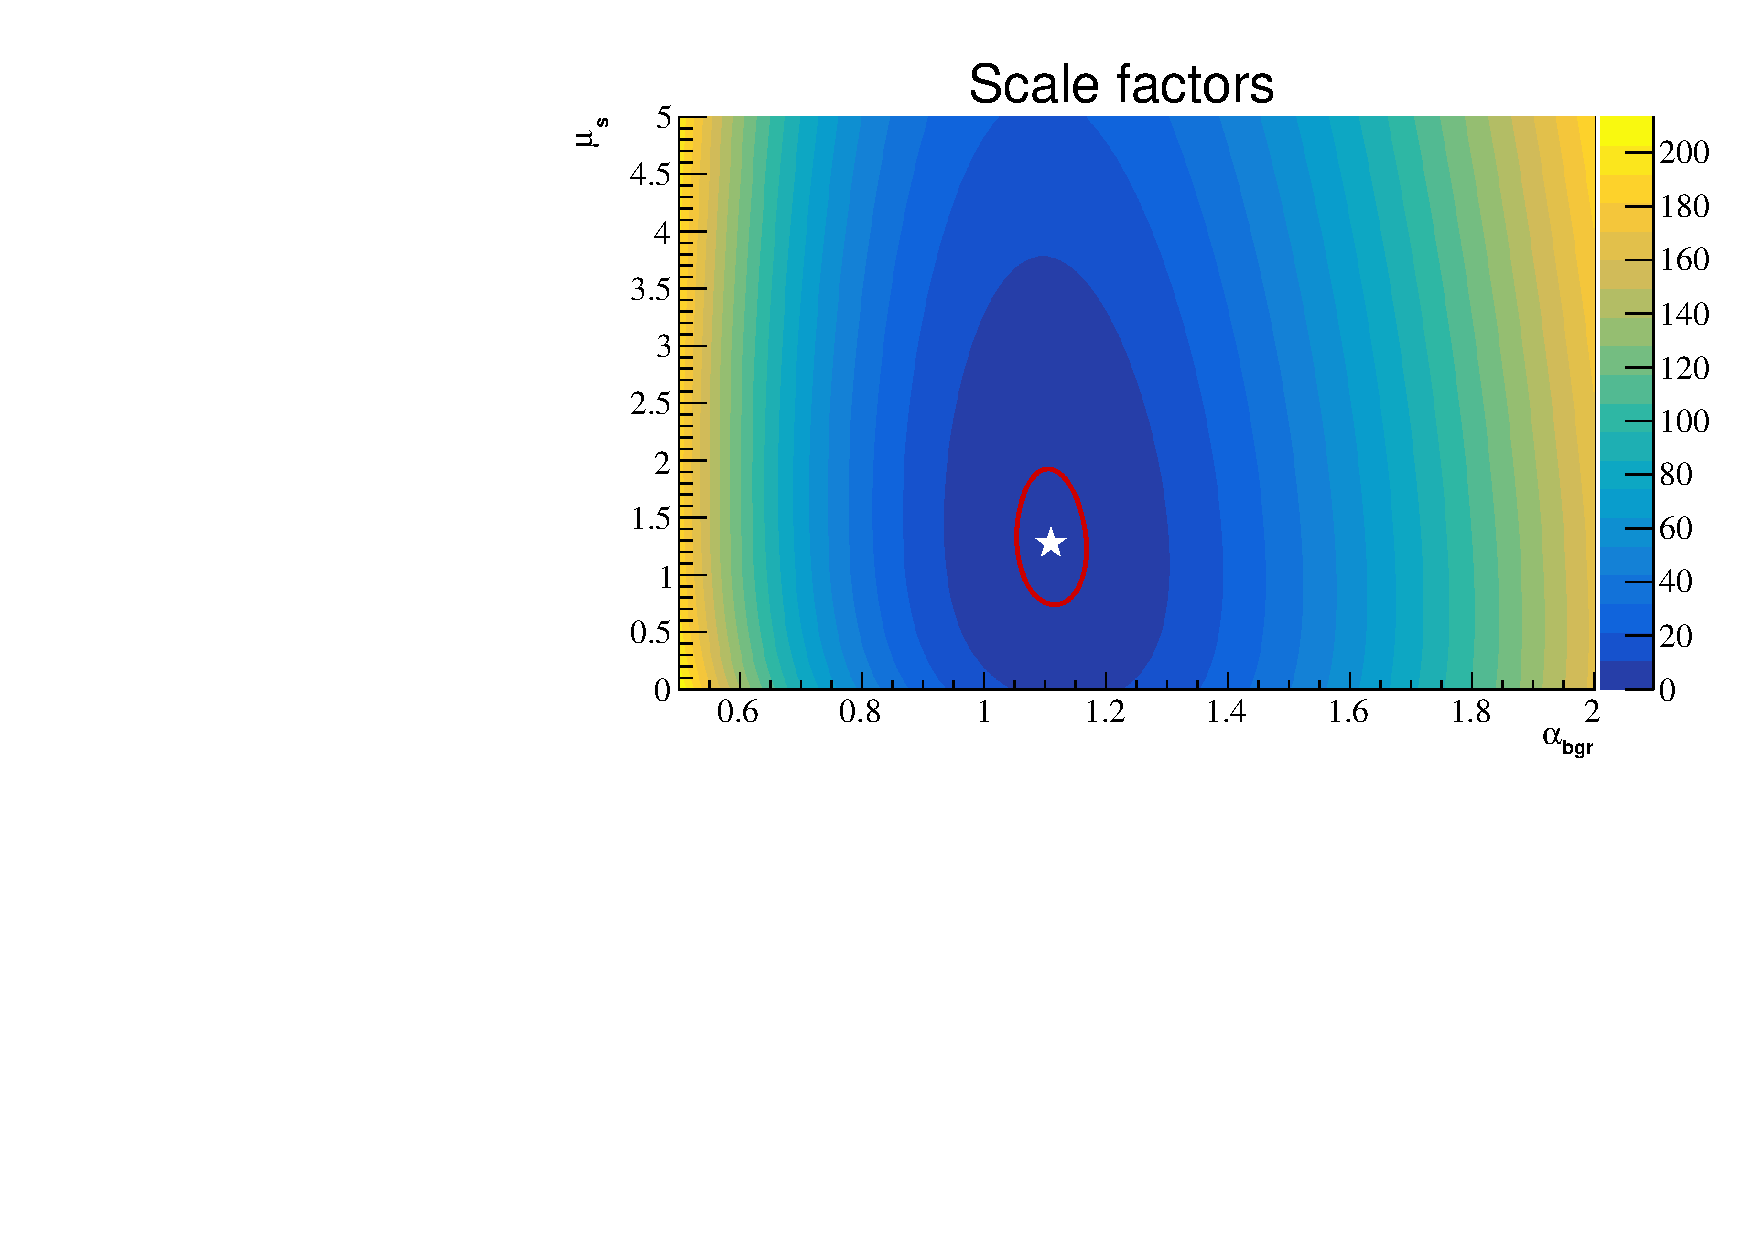
\includegraphics[width=0.8\textwidth]{../data/11_3/optimal_scale_factors_-2logL.pdf}
\caption{Contour plot of $-2\log(\mathcal{L})$ where the x-axis corresponds to the range of scale factors used for the background, the y-axis for the signal, while the z-axis with corresponding colorbar to the right corresponds to $-2\log(\mathcal{L})$. The red ellipse around the star is the corresponding $1\sigma$ uncertainty.}
\label{fig:optimal_scalefactors_contourPlot}
\end{figure}

\subsection{Computing the test-statistic} \label{subsec:Analysis-(computing the test-statistic)}
Using eq.~\eqref{eq:test_statistic}, where $H_0$ corresponds to our b-only hypothesis and $H_1$ corresponds to our $s+b$ hypothesis, and $\alpha_{bgr} = 1$ we obtain a test-statistic of
\begin{align}
t = -11.53
\end{align}
Since the test-statistic is negative this means that the likelihood of the data being provided by $H_1$ is greater than the likelihood of the data being solely explained by the $H_0$ hypothesis.

Through the use of MC toy-datasets we can generate a distribution of the number of simulated b-only and $s+b$ datasets vs. the calculated test-statistic. The distribution is produced by generating 20000 histograms and calculating the median test-statistic for each dataset. The test-statistics are then gathered in a separate histogram where each bin corresponds to the number of toy-data sets resulting in a given median test-statistic. From this we get the distribution as seen in figure~\ref{fig:toyMC_test_statistic}. The medians for the test statistic is given in table~\ref{tab:toyMC_test_statistic_median}.

\begin{table}[]
\caption{Median test statistics calculated from toy MC datasets for b-only and $s+b$.}
\label{tab:toyMC_test_statistic_median}
\begin{tabular}{cccc}
\hline\hline
       & b-only & $s+b$ & data\\ \hline
$t$ & 4.67   & -5.60   & -11.53    \\ \hline\hline
\end{tabular}
\end{table}

\begin{figure}
\centering
\includegraphics[width=0.8\textwidth]{../data/11_3/test_statistic_distribution.pdf}
\caption{Distribution of test-statistic vs. pseudo datasets generated by toy MC, where the green bands include 68\% of the toy datasets, while the yellow bands indicate the borders for which 95\% of the toy datasets are contained within.}
\label{fig:toyMC_test_statistic}
\end{figure}


\subsection{Discovery-aimed} \label{subsec:Analysis-(dicovery aimed)}
Using eq.\eqref{eq:1-CL_b} we can calculate the p-values for the median b-only, $s+b$ and data experiments.
As seen from table~\ref{tab:Significance_vs_lumScaleFactors} the p-value, $1-CL_b$, under the median test-statistic for the $s+b$ hypothesis with $\mu_s = 1.0$ is 0.0068 which results in an expected significance $Z_{exp} = 2.47\sigma$. The observed data however has a p-value of 0.1559, giving an observed significance $Z_{obs} = 3.72$. This means that since $Z_{exp} < 5\sigma$ we cannot make any claims of a discovery. Nor can we actually expect to make a discovery according to the observed significance, $Z_{obs} < 5\sigma$.

\subsection{Exclusion aimed} \label{subsec:Analysis-(exclusion aimed)}
Now using eq.~\eqref{eq:CL_s+b} we can find the exclusion limits from the confidence level $CL_{s+b}$. We see that the $CL_{s+b}$ for the b-only hypothesis is $0.0183 < 5\%$, which would imply that we can expect to exclude the $H_1$ hypothesis. While for the data we have that $CL_{s+b} = 0.5044 > 5\%$ which implies that we cannot exclude the signal hypothesis. However, as seen from figure~\ref{fig:toyMC_test_statistic}, the distributions of the $H_0$ hypothesis and the $H_1$ hypothesis are overlapping. Thus, in order to obtain a more accurate picture of the exclusion limits we can make use of the $CL_s$ method, as described in section~\ref{subsubsec:Theory-(p-values and significance)-(confidence-levels)}. As can be seen from table~\ref{tab:discovery_exclusion_confidence_levels}, $CL_s = 0.8444 > 0.05$ meaning that we cannot exclude the signal ($m_H = 125$ GeV) hypothesis.

However, what is also worth investigating is when we could expect to make an exclusion of the $H_1$-hypothesis as a function of the cross-sections. Since the number of events is proportional to the cross-section, assuming a constant luminosity scalefactor, we can increase the number of signal events by increasing $\mu_s$. As seen from table~\ref{tab:discovery_exclusion_confidence_levels}, we have for $\mu=2.75$ that $CL_s$ for the data test-statistic is $0.0970>5\%$, so we cannot yet make a claim of excluding $H_1$. However, as we reach a signal scalefactor $\mu_s \sim 3.50$ then $CL_s$ is now $0.0493<5\%$. Thus, at 3.50 times the amount of signal events we can expect to make an exclusion of $H_1$.

\begin{table}[]
\caption{Discovery and exclusion limits is shown below in the C.L. column along with the confidence level ratio $CL_s$ for the b-only and $s+b$ hypotheses as well as the data. The scaling factor $\mu_s$ implcitly represents the scaling of the cross-section.}
\label{tab:discovery_exclusion_confidence_levels}
\begin{tabular}{c|ccc|ccc|ccc}
\hline\hline
           & \multicolumn{3}{c|}{$\mu_s = 1.00$} & \multicolumn{3}{c|}{$\mu_s = 2.75$} & \multicolumn{3}{c}{$\mu_s = 3.50$} \\ \hline
$C.L.$     & b-only    & $s+b$     & Data      & b-only    & $s+b$     & Data      & b-only    & $s+b$     & Data     \\ \hline
$1-CL_b$   & 0.4989    & 0.0068    & 0.0001    & 0.4998    & 0.0000    & 0.0001    & 0.4996    & 0.0000    & 0.0000   \\
$CL_{s+b}$ & 0.0212    & 0.5016    & 0.8434    & 0.0000    & 0.5001    & 0.0972    & 0.0000    & 0.5008    & 0.0441   \\
$CL_s$     & 0.0423    & 0.8441    & 0.8435    & 0.0000    & 0.5001    & 0.0972    & 0.0000    & 0.5008    & 0.0441   \\ \hline\hline
\end{tabular}
\end{table}

\section{Conlcusions}
We have shown that in order to make any affirmative statement about the discovery of a signal one would require an increase of the luminosity scalefactor by $5.40$. We also found that, by the amount of data given, we cannot expect to make a discovery according to the expected significance, nor can we exclude the signal hypothesis based on the observed significance.


\printbibliography
\end{document}


